%************************************************
\chapter{Probability Theory}\label{ch:probability}

%************************************************
\openepigraph{A wise man proportions his belief to the evidence.}{David Hume}
In this chapter, propositional calculus and probability theory are derived from a list of desired characteristics for sceptical agents.

\section{From Language to Probability}\label{sec:language_probability}
\subsection{Formal Languages} We, as intelligent agents, do not know how the World is; we only know how we perceive it. Our ideas are mental pictures of how we imagine the World. Like in the story of the blind men and the elephant (\cref{blind_men}), how do we know that our model is the same as someone else's? \emph{Communicating}. We need to communicate with each other to check if our mental picture of the World, our model, is consistent with the experience of others.\footnote{We can take this idea further and think that at any moment we need to communicate with our past selfs to check if new evidence is consistent with our prior model.}.

We use language to describe the World. However, natural languages, like English, German, Portuguese, are ambiguous, and we need contextual clues and other information to more clearly communicate meaning. To avoid this, an intelligent agent uses formal language.

A formal language is a mathematical tool created for precise communication about a specific subject. For example, arithmetic is a language for calculations. Chemists have a language that represents chemical structures of molecules. Programming languages are formal languages that express computations. In a nutshell, a formal language is a set of words (strings) whose letters (symbols) are taken from an alphabet and are well-formed according to a specific set of rules, a grammar:
\begin{align}
	\text{Let }\lang&= <\Sigma, \Phi>,~\text{be a formal language where:}\\
	\Sigma &= \{S_1, S_2, \cdots, S_n\} \text{ is an alphabet,}\\
	\Phi &= {\Phi_1 \cup \Phi_2 \cup \cdots \cup \Phi_k} \text{ is a set of operations,}
\end{align}
where:
\begin{align}
	\Phi_1 &\text{ is the set of unary operations}, \nonumber\\
	\Phi_2 &\text{ is the set of binary operations}, \nonumber\\
	\cdots &\nonumber \\
	\Phi_k &\text{ is the set of k-ary operations}\nonumber
\end{align}
A formal language allows a quantitative description of a state of knowledge and defines how this state can be updated on new evidence.

With this definition, we can also think that a formal language is what~\citeauthor{sowinski:2016} calls a \emph{realm of discourse}, \ie all the valid formed \emph{strings}\footnote{Strings, words, sentences, propositions, formulae are names used interchangeably through the literature.} that one can derive; everything one can \emph{say} about the world.

Interestingly, formal languages allow us to manipulate representations of the world without dealing with their semantics. They are the basis of \emph{``Turing's strange inversion''}, (see \cref{turing_strange_inversion}) by doing allowed operations on strings, computers can compute at a superhuman speed and accuracy without ever comprehending what they are doing.

\subsection{From Rationalism to Propositional Calculus}
\paragraph{Rational Agents} Rational agents are agents that can form representations of a complex world, use deduction as the inference process to derive updated representations, and use these new representations to decide what to do. In other words, rational agents are the consequence of the epistemological view of \emph{rationalism}.

When a particular statement's truth value is established by a rational agent, all statements formed in her knowledge base from that statement instantly feel that update. A rational agent cannot hold contradictions.

\paragraph{Desiderata for a rational language}\label{sec:desiderata_language}

We want to build a language for rational agents with the following desired characteristics:
\begin{enumerate}
	[I.]
	\item \textbf{knowledge is absolute}; a sentence\footnote{A sentence can be either a single symbol or a string formed with several symbols according to the grammar.} can be either true or false;
	\item \textbf{unambiguous}, a constructed sentence can only have one meaning;
	\item \textbf{consistent}; a language without paradoxes, \ie whatever path chosen to derive a sentence truth value will lead to the same assignment;
	\item \textbf{minimal}; uses the smallest set of symbols possible.
\end{enumerate}

Let \(\lang_R= <\Sigma_R, \Phi_R>\) be the formal language built from these constraints; where sentences are either axiom symbols or compounded sentences formed using special symbols called operators, each operator denoting one operation \(\phi \in \Phi_R\).

It is possible to prove\label{future:prove_minimal_language_logic} that \(\lang_R\) only needs one operator~\cite{sowinski:2016,jaynes:2003}: \spacedlowsmallcaps{nand} (or \spacedlowsmallcaps{xor}), and it is also equivalent to Propositional Calculus.\footnote{Proposition is synonym to sentence, and Propositional Calculus is also known as Sentential Calculus.}.~\label{insert_appendix} In other words, Logic is the language that emerges from our desiderata, from rationalism. \textbf{Logic is the language of mathematics}.

A point worth mentioning is that using Logic as an agent formal language means the \textbf{implicit acceptance} of the constraints above.

\subsection{From Empiricism to Probability Theory}

The constraints that lead to Logic are very restrictive to use in the real world; the rational language has a comparatively small realm of discourse. Hume would say that it is only helpful for \emph{relations of ideas}, talking in the abstract, and not for \emph{matters of facts}, talking about reality.

A realm of discourse to talk about reality needs at least the empiricist perspective where knowledge is justified belief, and that one should \emph{weights her beliefs to the evidence.} The quantity that specifies to what degree we believe a proposition is true is constrained by other beliefs, i.e.\ by previous experience and evidence gathering.

\paragraph{Sceptical Agents}\label{sec:sceptical_agent}\label{sec:sceptical_agents} In the sceptical agent derived from the empiricist epistemology
(authors have called these agents epistemic agents~\cite{caticha:2008}, idealised epistemic agents~\cite{sowinski:2016} or robots~\cite{jaynes:2003}), beliefs are not independent of each other~\cite{caticha:2008}, they form an interconnected web that is the agent's knowledge base. The update mechanism, its inference method, follows the principle of minimality, i.e.\ it tries to minimise the change in the knowledge base.

\paragraph{Desiderata for a sceptical language} As we did for rational agents, let us state a set of desired characteristics for the language of Science, \(\lang_S= <\Sigma_S, \Phi_S>\)
\footnote{~\citeonly{sowinski:2016,caticha:2008, jaynes:2003} also present this same idea of deriving probability theory from a desiderata.}:
\begin{enumerate}[I.]
	\item \textbf{Knowledge is a set of beliefs, quantifiable by real numbers and dependent on prior evidence:~\cite{sowinski:2016,caticha:2008, jaynes:2003}}\footnote{Moacir: is this yours formulation?} \\
	Let \(S_i \in \Sigma_S\) be sentences about the world. Given any two statements \(S_1\), \(S_2\), the agent must be able to say that \(S_1\) is more plausible than \(S_2\), or that \(S_2\) is more plausible than \(S_1\), or that \(S_1\) and \(S_2\) are equally plausible~\cite{caticha:2008}. Thus we can list statements in an increasing plausibility order. Real numbers can represent this transitive ordering~\cite{caticha:2008}.\footnote{We are implicitly assuming that the language we are building has infinite statements. A further discussion on this continuity assumption can be found in~\cite[p. 26]{sowinski:2016}}.

	Let \(b\) be a measure of degrees of belief in \(S\) given some previous knowledge \(K\):\footnote{Moacir: K --- is it an (observable) event? or knowledge/axiom?}
	\footnote{Using \((S|K)\) in a function is a notation abuse that we accept in order to better explain the idea.}:
	\begin{align}
		b: \Sigma_S \to \Real\\
		b: S \mapsto b(S|K)
	\end{align}
	Here we capture the fact that plausibility (degrees of belief) is not a function of a sentence, but a relation between a sentence and a given assumed prior knowledge.
	\item \textbf{``Common sense:''}\\
	The plausibility of compound sentences should be related by some logical function to the plausibility of the sentences that form them. \\
	We already showed that a minimal rational language has only one operator. Here, instead of using the \spacedlowsmallcaps{nand} operator, for a matter of familiarity, let us use the almost minimal language with the operators \spacedlowsmallcaps{not} (\(\neg\)) and \spacedlowsmallcaps{and} ($\land$). In this setting, we are saying there are such functions $f$ and $g$ that~\cite{sowinski:2016}:
	\begin{enumerate}[(a)]
		\item \(b(\neg S|K) = f[b(S|K)]\)
		\item \(b(S_1 \land S_2 | K) =\\g[b(S_1|K), b(S_1|S_2), b(S_2|K), b(S_2|S_1)]\)
	\end{enumerate}
	\item \textbf{Consistency:}\\
	The functions \(f\) and \(g\) must be consistent with the grammar \(\Phi\) (production rules).\\Consistency guarantees that whatever path used to compute the plausibility of a statement in the context of the same knowledge web (the same set of constraints) must lead to the same degree of belief.\label{consistency}
	\begin{enumerate}
		[(a)]
		\item Beliefs that depend on multiple propositions cannot depend on the order in which they are presented.\label{axiom:order}
		\item No proposition can be arbitrarily ignored.
		\item Propositions which are known to be identical must be assigned the same degree of belief.
	\end{enumerate}
\end{enumerate}
\sidefigure{kolmogorov}{-20}{Andrey Kolmogorov, Soviet mathematician.}

Such desiderata have a name; it is known as Cox's axioms, and one can derive the Sum Rule and the Product Rule (see \cref{sec:probability}) from them, therefore, also the Bayes' Theorem (\cref{sec:bayes_theorem}), and reverse-engineer Kolmogorov's Axioms of Probability Theory (\cref{sec:kolmogorov_axioms}, \cref{fig:kolmogorov})\label{future:cox_to_kolmogorov}~\cite{sowinski:2016, jaynes:2003, caticha:2008, terenin:2015}.

In other words, Probability Theory is the language that emerges from our desiderata, from empiricism. \textbf{Probability theory is the logic of science}~\cite{jaynes:2003}, and our measure \(b\) is what is usually called probability~\(P\).

Again, here we explicit that by using Bayesian inference to build and communicate concepts of the world (models), we are assuming Cox's axioms above.

\subsection{Assumptions and their consequences} As a side note, let us take this opportunity to explore what some assumptions mean to human intelligence in particular. It is indisputable\footnote{Unless you are an economist.} that humans are not rational, neither sceptical agents. The whole idea of imagining a sceptical agent is a consequence of wanting to address intelligence without the human complexities.

However, are humans irrational because of biology or psychology? Are we irrational for lack of will, or could it be that Nature wires the human brain in a way that pr\emph{events} us from following these axioms? Here we argue that biology has an important role. Researchers have found, for instance, that visual acuity can be permanently impaired if there is a sensory deficit during early post-natal development~\cite{wiesel:1982}. If the human brain is not exposed to some samples in its infancy, it will never achieve the accuracy level it could achieve if it had experienced them, regardless of experiencing those examples later. In other words, \emph{human beliefs depend on the order in which pieces of evidence are presented}, contradicting Cox's axiom~\ref{axiom:order}.


\section{Formalizing Probability Theory} Up to this point in the chapter, our purpose was to give an intuition of what probability is. We did that by showing that it is possible to derive Kolmogorov's Axioms (\cref{sec:kolmogorov_axioms}) from the empiricist epistemology. In this section, we will use these axioms to derive concepts in Probability Theory.

Worth of mention, several concepts in this section are \emph{relations of ideas}, not \emph{matters of fact}. The probability of an \emph{event} E, P(E), can be computed by marginalisation (see Subsection~\ref{marginalisation}), but as discussed before, there are no beliefs in a vacuum. In reality, there is only the probability of an \emph{event} E given some background knowledge \(K\). This change of epistemological perspective is essential to be remembered now; that we will expose the idealised development of concepts in Probability Theory.


\section{Experiments, Sample Spaces and Events}

The set of possible outcomes of an \textbf{\emph{experiment}} is the \textbf{sample space} \(\Omega\). Let us use the canonical \emph{experiment} of rolling a dice. In this experiment, the sample space is:
\begin{align*}
	\Omega = \left\{\epsdice{1},\epsdice{2},\epsdice{3},\epsdice{4},\epsdice{5},\epsdice{6} \right\}
\end{align*}
An \textbf{outcome} or \textbf{realization} is a point $\omega \in \Omega$:
\begin{align*}
	\omega_3&=\epsdice{3}\\
	\Omega &= \left\{\omega_1=\epsdice{1},\cdots,\omega_6=\epsdice{6} \right\}.
\end{align*}
An \textbf{Event} is something you can say about the \emph{experiment}, \eg ``The dice rolled to the an odd number''. It is a true proposition. But easier than writing so much, we denote \emph{events} with letters. \textbf{Events are subsets of \(\Omega\)} (see \cref{fig:event_A}).
\begin{align*}
	A &= \left\{\va_1=\epsdice{1}, \va_2=\epsdice{3}, \va_3=\epsdice{5} \right\}\\
	A &\subset \Omega
\end{align*}
We say that $A_1, A_2, \cdots$ are \textbf{mutually exclusive} or \textbf{disjoint} \emph{events} if $A_i \cap A_j=\emptyset, \forall i\neq j$. For example, \(A\) is the \emph{event} ``the dice rolled to the value 5'' and \(B\) is the \emph{event} ``the dice rolled to an even number''. In this case, \(A\) and \(B\) are disjoint (see~\cref{fig:disjoint_events})
\begin{figure}
	[hbt!] \centering
	\begin{subfigure}
		[t]{.3
		\textwidth} \centering
		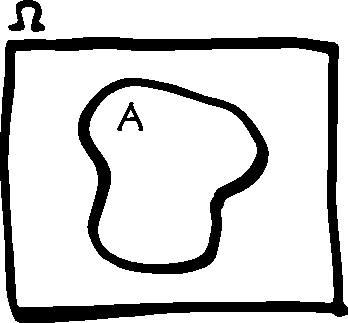
\includegraphics[width=3cm]{eventA}
		\caption{An \emph{event} \(A\).}\label{fig:event_A}
	\end{subfigure}
		\hfill
	\begin{subfigure}
			[t]{.3
			\textwidth} \centering
			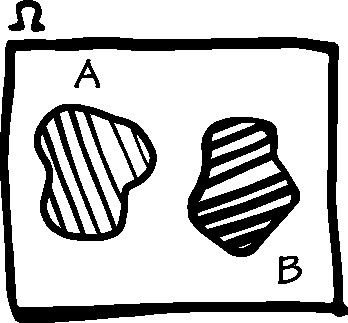
\includegraphics[width=3cm]{disjointAB}
			\caption{Disjoint events \(A\) and \(B\): \(A \cap B = \emptyset\).}\label{fig:disjoint_events}
	\end{subfigure}
	\hfill
	\begin{subfigure}
		[t]{.3
		\textwidth} \centering
		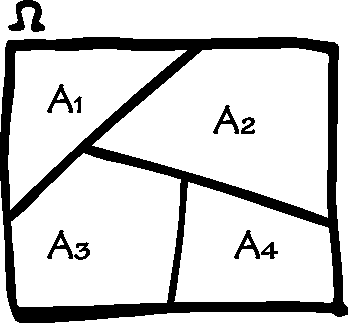
\includegraphics[width=3cm]{partition}
		\caption{A partition of \(\Omega\):\\
		\(\bigcup\limits_{i}^{} A_i = \Omega\).}\label{fig:partition}
	\end{subfigure}
	\caption{Events, disjoint events and partitions.}
\end{figure}
A \textbf{partition} of $\Omega$ is a sequence of disjoint events (sets) \(A_i\) (see~\cref{fig:partition}), where:
\begin{align}
	A_1, A_2, \cdots A_i \text{ s.t. } (A_1 \cup A_2 \cup A_3 \cdots = \bigcup\limits_{i=1}^{\infty} A_i) = \Omega
\end{align}


\section{Probability}\label{sec:probability}
\marginnote{The powerset of \(\Omega\), \(\powerset(\Omega)\), is the set of all possible subsets of \(\Omega\).}
\begin{definition}[Kolmogorov's Axioms]\label{sec:kolmogorov_axioms}
	A function \(P: \powerset(\Omega) \to \sR \) that maps any \emph{event} \(A\) to a real number \(P(A)\) is called the \textbf{probability measure} or a \textbf{probability distribution} if it satisfies the Kolmogorov's axioms~\cite{wasserman:2013}:
	\begin{enumerate}[\textbf{Axiom} 1., leftmargin=3cm]
		\item \(P(A)\geq 0, \forall A\)
		\item \(P(\Omega)=1\)
		% \item If \(A\) and \(B\) are disjoint, i.e. \(A \ind B \),\label{axiom:disjoint}
		\begin{align}
			P(A \lor B)= P(A)+P(B)\label{eq:sum_rule} \\
			\nonumber \tag{Sum Rule}
		\end{align}
	\end{enumerate}
\end{definition}

Visually, we can represent the probability of an \emph{event} \(A\), \(P(A)\), as the proportion of the sample space, the \emph{event} occupies. To diferentiate \emph{events} from their probabilities, we will shade the area of the \emph{event}.
\begin{figure}[ht!]
\captionsetup[subfigure]{labelformat=empty}
\begin{sidecaption}[Kolmogorov's Axioms and their direct consequences.]{Kolmogorov's Axioms and their direct consequences.}\label{fig:kolmogorov_axioms}
\centering
\begin{subfigure}[t]{.3\textwidth}\centering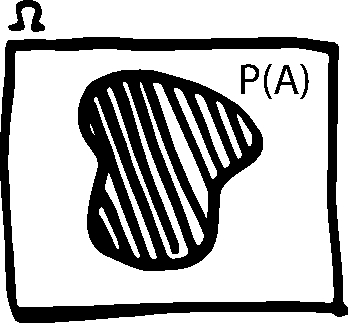
\includegraphics[width=3cm]{pA.pdf}
	\caption{Axiom 1: \\\(P(A)\geq 0\)}\label{fig:axiom1}
\end{subfigure}
\hfill
\begin{subfigure}[t]{.3\textwidth} \centering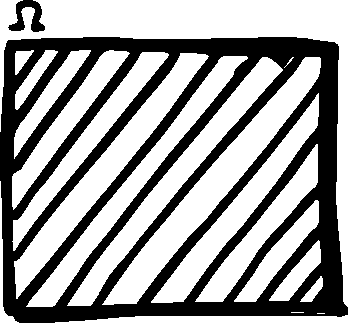
\includegraphics[width=3cm]{p1}
	\caption{Axiom 2:\\\(P(\Omega)=1\).}\label{fig:axiom2}
\end{subfigure}
\hfill
\begin{subfigure}[t]{.3\textwidth} \centering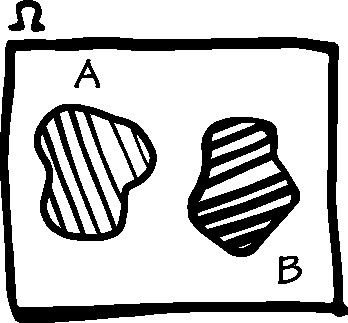
\includegraphics[width=3cm]{disjointAB}
	\caption{Axiom 3: \(A \cap B = \emptyset \implies P(A \lor B)=P(A)+P(B)\).}\label{fig:axiom3}
\end{subfigure}
\hfill
\begin{subfigure}
[t]{.3
\textwidth} \centering

\includegraphics[width=3cm]{emptyspace}
\caption{\(P(\emptyset)=0\).}
\end{subfigure}
\hfill
\begin{subfigure}
[t]{.3
\textwidth} \centering
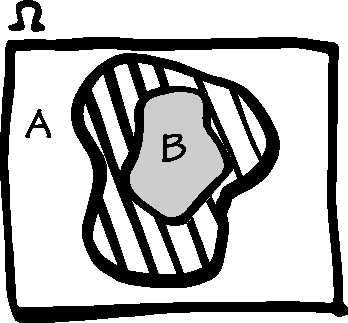
\includegraphics[width=3cm]{BinA}
\caption{\(B\subset A \to P(B) \leq P(A)\).}
\end{subfigure}
\hfill
\begin{subfigure}
[t]{.3
\textwidth} \centering
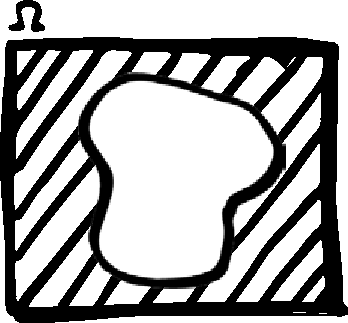
\includegraphics[width=3cm]{complementA}
\caption{\(P(\bar{A})=1-P(A)\).}
\end{subfigure}
\end{sidecaption}
\end{figure}

Directly from the Kolmogorov Axioms, one can derive~\cite{jaynes:2003} other properties (see \cref{fig:kolmogorov_axioms_derivations}):
\begin{align}
P(\emptyset)&=0\\
B \subset A &\implies P(B) \leq P(A)\\
0 &\leq P(A) \leq 1\\
P(\bar{A})&=1-P(A).
\end{align}



\section{Joint event}
\begin{definition}
A joint \emph{event} \(A, B\) is the set of outcomes where:
\[(A, B) = {\omega \in \Omega: (\omega \in A \cap B) } \]
Therefore,
\[P(A, B) =P({\omega \in \Omega: (\omega \in A \cap B) }) \]
\end{definition}
\marginnote{\vspace{-2cm}
\begin{align}
&P(A,B) &~\equiv~ &P(B,A)&~\equiv~ \nonumber\\
&P(A \land B)&~\equiv~ &P(A \cap B)&~\equiv~  \nonumber\\
&P(A \times B).\nonumber
\end{align}
}
When talking about \emph{events} as propositions, it is straightforward to use logic notation \(P(A \land B)\), but when we start to use \emph{random variables} (\cref{sec:random_variables}), we will adopt the shorthand notation \(P(\rvA, \rvB)\).
\sidefigure{joint_event}{0}{Joint event (A, B).}

\section{Independent events}\label{sec:independent_events}
\begin{definition}\label{def:independence}
Events \(A\) and \(B\) are \textbf{independent} (\(A \ind B\)) if:
\begin{align}
A\neq \emptyset, B\neq \emptyset \implies P(A)>0, P(B)>0\label{eq:P(A, B)>0}\\
P(A, B) = P(A \land B) = P(A) \cdot P(B)\label{eq:Product_Rule}\\
\nonumber \tag{Product Rule}
\end{align}
\end{definition}

\textbf{Disjoint \emph{events} cannot be independent}, since (from~\eqref{eq:P(A, B)>0}) \(P(A) \cdot P(B)> 0\), but as disjoint \emph{events} (\cref{fig:disjoint_events}) \(P(A \land B)=P(\emptyset)=0\), leading to contradiction.

Independence can be assumed or derived by verifying:
\begin{align}
P(A \land B)= P(A) \cdot P(B).\\
\nonumber \tag{Independent variables}
\end{align}


\section{Conditional probability}
\marginpar{
\centering
\begin{gather*}
P(A|B)=\frac{ 
\includegraphics[width=2cm]{eventAB} }
{ 
\includegraphics[width=2cm]{eventB}}
\end{gather*}
}
% \begin{wrapfigure}{R}{0.27\textwidth}
% 	\centering
% 	\begin{gather*}
% 		P(A|B)=\frac{ 
\includegraphics[width=2cm]{eventAB} }
% 		 						{ 
\includegraphics[width=2cm]{eventB}}
% 	\end{gather*}
% \end{wrapfigure}
As we have explained before (\cref{sec:sceptical_agent}), the plausibility of an outcome or a set of outcomes depends on a web of interconnected prior beliefs. So, in reality, as a \emph{matter of fact}, what exists are probabilities \emph{conditional} to a given prior assumption.

\begin{definition}
If \(P(B)>0\) then the \textbf{conditional probability} of A given B is:
\begin{align}\label{eq:conditional_probability}
P(A|B) \eqdef \frac{P(A,B)}{P(B)}
\end{align}
Also:
\begin{align}\label{eq:joint_probability}
P(A, B) \eqdef P(A|B)\cdot P(B)
\end{align}
\end{definition}


Except if \(P(A) \equiv P(B)\), \(P(A|B) \neq P(B|A)\). Also, \(P(A|B)=P(A) \iff A \ind B\).\footnote{Venn diagrams are not helpful to see that the \emph{events} are independent, as it all depends on the areas of intersection and the sizes of A and B, which are quite difficult to estimate without computational help.}.

\section{Marginal probability}\label{marginalisation}
\begin{theorem}
Let \(A_1, \cdots, A_k\) be a partition of \(\Omega\). Then, for any \emph{event} B,
\begin{align}
P(B)=\sum_{i=1}^k P(B|A_i)\cdot P(A_i)\label{eq:law_of_total_probabilities} \end{align}
\end{theorem}
\blockfigure{total_probability}{1}{An \emph{event} B, a partition \(A_i\) over \(\Omega\), and \(C_i = (B, A_i) \).}

\begin{proof}
\footnote{Remember: \((B, A) \equiv (B \cap A)\).}
Define \(C_i = (B,A_i)\). Let \(C_1, \cdots C_k\) be disjoint and \(B = \bigcup\limits_{i=1}^k C_i\). \\
Therefore:

	\begin{align}
		P(B) &\triangleq P(\bigcup\limits_{i=1}^k C_i)
		\overset{\text{\ref{eq:sum_rule}}}{=} \sum_i P(C_i)\\
		&\triangleq \sum_i P(B,A_i)
		\overset{\text{\ref{eq:conditional_probability}}}{=} \sum_{i=1}^k P(B|A_i)\cdot P(A_i) \tag{Law of Total Probability}
	\end{align}
\end{proof}
\section{Bayes' theorem}\label{sec:bayes_theorem}
\begin{theorem}
	Let \(A_1, \cdots, A_k\) be a partition of \(\Omega\) s.t. \(P(A_i)>0, \forall i\) then, \(\forall i=1, \cdots, k\):
	\begin{align}
		P(A_i|B)= \frac{P(B|A_i)\cdot P(A_i)}{\sum_i P(B|A_i)\cdot P(A_i)} \tag{Bayes' theorem}
	\end{align}
\end{theorem}
\begin{proof}
	From equations~\ref{eq:conditional_probability},~\ref{eq:joint_probability} and~\ref{eq:law_of_total_probabilities}:
	\begin{align}
		P(A_i|B)&\overset{\text{\ref{eq:conditional_probability}}}{=}\frac{P(A_i,B)}{P(B)} \overset{\text{\ref{eq:joint_probability}}}{=} \frac{P(B|A_i) \cdot P(A_i)}{P(B)}  \\
		&\overset{\text{\ref{eq:law_of_total_probabilities}}}{=}\frac{P(B|A_i)\cdot P(A_i)}{\sum_{i=1}^k P(B|A_i)\cdot P(A_i)}
	\end{align}
\end{proof}
We call \(P(A_i)\) the \textbf{prior} of A, and \(P(A_i|B)\) the \textbf{posterior} probability of A.
\section{Random variables}\label{sec:random_variables}
\begin{definition}
	A \textbf{random variable} is a mapping \(\rvX:\Omega \to \Real\) that assigns a real number \(\rvX(\omega)\) to each outcome \(\omega\), \(\omega \mapsto \rvX(\omega)\).
\end{definition}
\sidefigure{random_variable}{0}{Random variable.}

Given a random variable \(\rvX\), the probability of an outcome \(\rx\) can be expressed as:
\begin{align}
	P(\rvX=\rx) = P(\rvX^{-1}(\rx)) = P(\{\omega \in \Omega: \rvX(\omega)=\rx\})\label{eq:P(X=x)} \end{align}

Several works on Probability Theory choose to start by defining random variables, rarely mentioning sample spaces, \emph{events} or the connection with logical propositions.

This usual approach is, nevertheless, confusing. Beyond the fact that random variables are not variables, but functions; nor random, they model uncertain \emph{events}; it is hard to grasp what random variables are without understanding their reasons for being.

The difference between a random variable $\rvX$ and a ``realization'' of it is the difference between a distribution and a sample from that distribution. In particular, a random variable $\rvX$ is ``formalized'' in terms of a function from the sample space to some result space, typically $\Real$. The realization of a random variable is ``what you get'' when an \emph{experiment} is run, and you figure out which \emph{events} happened, and you apply $\rvX$ to those \emph{events}.

\subsection{Notation hell} If a \emph{random variable} is a function, how can we write \(P(\rvX=4)\) or \(P(\rvX > 7)\)? The reason for such confusion is due to some notation abuse that became standard in works on probability theory. It is not easy to grasp it in the beginning, but the explanation was already stated at~\eqref{eq:P(X=x)}. \(P(\rvX=\rx)\) is a shorthand for \(P(\rvX^{-1}(\rx))\).

Technically, a \emph{random variable} is a function.  In practice, it is just a mathematical tool to help us associate propositions with numbers. It is called a \emph{random variable} because the notation abuse treats the function as a variable.

To help clear up such confusion, let us recap a little the notation we have established before:

In the canonical \emph{experiment} of rolling a dice, instead of writing the plausability of the proposition \emph{``The dice will roll to number 4''} is \(\frac{1}{6}\), it is easier to assign a letter to the proposition, or as we called the \emph{event}. Let us use \emph{event} \(D\) to represent the proposition. Then, we can use \(P(D)=\frac{1}{6}\). Now, we are going one step further, instead of using the \emph{event} \(D\) we use the \emph{random variable} \(\rvD\), in italic, and say \(P(\rvD=4)=\frac{1}{6}\).

Notice the difference between a \emph{random variable} and an \emph{event}
% .\footnote{An \emph{event} can be seen as a special kind of \emph{random variable}.  \Eg, a random variable \(\rvD\) is the truth function (also known as the indicator function) over an event \(D\):
% \begin{align*}
% 	\rvD=\truth_D
% \end{align*}
% That is the reason one can say that ``\emph{random variables} define \emph{events}.'' }
: \(\rvD\) could assume any value (even \(\rvD=7\) which is clearly outside of our \emph{sample space}). Would it not be easier then to use an index to the \emph{event} letters, \ie \(D_4\) to value 4, and \(D_1\) to value 1, etc.? Not really.

Besides providing this shorter notation, the mapping of the random variable allows us to manipulate \emph{events} as numbers: for example, we can chart probability distributions using random variables, which we cannot cope with \emph{events}.


\section{Probability Distributions}
\sidefigure{distribution}{0}{Probability mass function, probability density function, and probability of an interval (hatched area).}

\begin{definition}
	A probability distribution of a discrete random variable \(\rvX\) or \textbf{probability mass function (pmf)} is a function \(p: \Omega \to [0,1]\) that provides the probabilities of occurrence of different possible outcomes in an \emph{experiment} (sample space):

	\begin{align}
		p(\rx) = P(\rvX = \rx), \tag{pmf}
	\end{align}
\end{definition}

If \(\rvX\) is countinuous, \(P(\rvX=\rx)\to 0\), therefore we need to use intervals in this case.
\begin{definition}
	A probability distribution of a countinous random variable \(\rvX\) in an interval \(A\), or \textbf{probability density function (pdf)} is a function \(p(\rx)\) that measures the probability of randomly selecting a value within the interval \(A=[a, b]\), as the area under its curve for the interval A:\@
	\begin{flalign}
		P(A) &= P[a \leq \rvX \leq b] = \int_{a}^{b} p(\rx) \, d\rx, \text{ and:}\\
		&
		\begin{cases}
			p(\rx) \geq 0, \forall x \tag{pdf}\\
			\int\limits_{\Real}^{} p(\rx) \, d\rx = 1
		\end{cases}
	\end{flalign}
\end{definition}
Now that we explained what distributions are,\footnote{In this dissertation, we will use $P(\rvX)$ to express the probability of a random variable, and $p(\rx)$ to represent a \emph{pmf} or \emph{pdf} of the random variable outcomes.} here we highlight some useful distributions:
\subsection{Statistical model}\label{sec:statistical_model}
A statistical model is a function $p_{\theta}(\rx) \equiv p(\rx | \theta)$ that represents the relationship between a parameter\footnote{In this dissertation we are interested in vector-valued $\theta$.} $\theta$ and potential outcomes $\rx$ of a random variable $\rvX$. In practice, we normally define a statistical model of a stochastic process for which we do not the real distribution. Therefore, the parameter $\theta$ has to be inferred from the observed data.
\subsection{Uniform distribution}\label{sec:uniform_distribution}
\marginpar{
	\begin{minipage}{\marginparwidth}
		\centering
		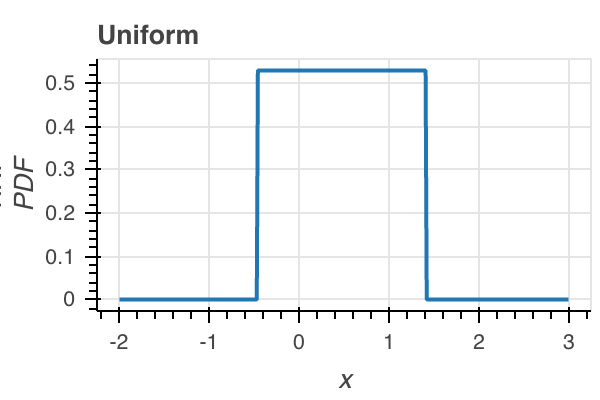
\includegraphics[width=0.9\textwidth]{uniform}
		\captionof{figure}{Uniform distribution.}\label{fig:uniform_distribution}
		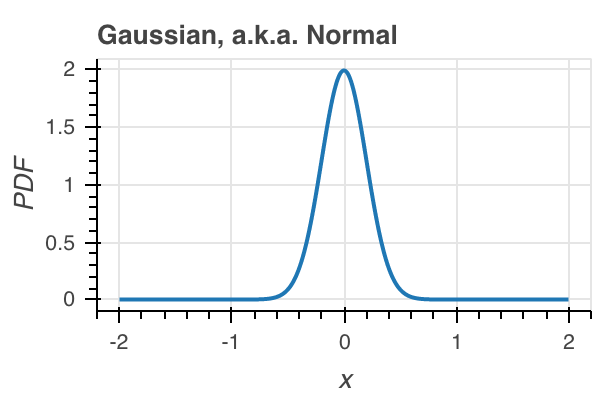
\includegraphics[width=0.9\textwidth]{gaussian}
		\captionof{figure}{Gaussian distribution, also known as the \emph{normal}.}\label{fig:gaussian_distribution}
		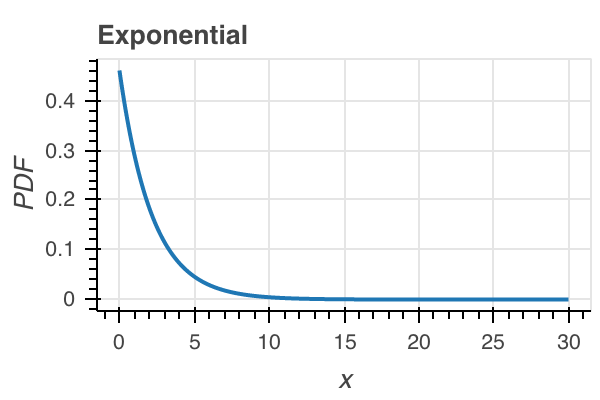
\includegraphics[width=0.9\textwidth]{exponential}
		\captionof{figure}{Exponential distribution.}\label{fig:exponential_distribution}
	\end{minipage}
}
\(\nonumber \\\rvX \sim \text{Uniform}(a,b)\), if:\\
\begin{align*}
	p(\rx)=
	\begin{cases}
		\frac{1}{b-a} & x \in [a,b]\\
		0 & \rx \notin [a,b]
	\end{cases}
\end{align*}
\subsection{Normal distribution}
\(\nonumber \\\rvX \sim N(\mu, \sigma^2)\), if:
\begin{align*}
	p(\rx)=\frac{1}{\sigma \sqrt{2\pi}}\exp{\Biggl{\{}{-\frac{1}{2\sigma^2}{(x-\mu)}^2}\Biggr{\}}}, \\~x \in \Real \\
\end{align*}
where \(\mu \in \Real\) (mean) and \(\sigma > 0\) (standard deviation). We say that \(\rvX\) has a \textbf{standard Normal distribution} if \(\mu = 0\), \( \sigma =1\).
\subsection{Exponential distribution}
\(\rvX \sim \text{Exp}(\lambda)\), if:
\begin{align*}
	p(\rx;\lambda) =
	\begin{cases}
		\lambda e^{-\lambda \rx} & \rx \ge 0, \\
		0 & \rx < 0.
	\end{cases}
\end{align*}
where \(\lambda > 0\) is the \emph{rate parameter} of the distribution.

\section{Joint Distributions}
\sidefigure{joint_distribution}{0}{A chart of a joint distribution.}
\begin{definition}
	Given a pair of discrete random variables \(\rvX\) and \(\rvY\), we define the \textbf{joint mass function} by \(p(\rx, \ry)=P(\rvX=\rx,\rvY=\ry)\).
\end{definition}
\begin{definition}
	Given a pair of continuous random variables \(\rvX\) and \(\rvY\), we define the \textbf{joint density function} by \(p(\rx, \ry)\), where:
	\begin{enumerate}
		[i.]
		\item \(p(\rx, \ry) \geq 0\)
		\item \(\bigintssss_{-\infty}^{\infty}\bigintssss_{-\infty}^{\infty}p(\rx,\ry) \, d\rx d\ry =1\)
		\item \(\forall A \subset \Real \times \Real, P((\rvX,\rvY)\in A)=\bigintssss\bigintssss_{A}p(\rx,\ry)\, d\rx d\ry \).
	\end{enumerate}
\end{definition}


\section{Expectancy, Variance and Covariance}
\begin{definition}
	The \textbf{expected value} or \textbf{mean} of \(\rvX\) is:
	\begin{align}
		\E (\rvX)=\langle \rvX \rangle = \SumInt_x \rx~p(\rx)~dx = \mu = \mu_X
	\end{align}
\end{definition}
\begin{theorem}
	Let \(\rvX_1, \cdots, \rvX_n\) be random variables and \(a_1, \cdots, a_n\) be constants, then from the \emph{Sum Rule}:
	\begin{align}
		\E \biggl(\sum_i a_i\rvX_i\biggr)=\sum_i a_i(\E (\rvX_i))
	\end{align}
\end{theorem}
\begin{theorem}
	Let \(\rvX_1, \cdots, \rvX_n\) be independent random variables, then from the \emph{Product Rule}:
	\begin{align}
		\E (\prod_i \rvX_i)=\prod_i \E (\rvX_i)
	\end{align}
\end{theorem}
\begin{definition}
	Let \(\rvX\) be a random variable with mean \(\mu\). The \textbf{variance} of \(\rvX\) is defined by:
	\begin{align}
		\sigma^2 = \sigma_{\rvX}^2 =\E {(\rvX - \mu)}^2
	\end{align}
	assumming this expectation exists. The standard deviation is \(\sigma\).
\end{definition}
\begin{definition}
	Let \({\rvX}\) and \({\rvY}\) be random variables with means \(\mu_{\rvX}\) and \(\mu_{\rvY}\), and with standard deviations \(\sigma_{\rvX}\) and \(\sigma_{\rvY}\). The \textbf{covariance} between \({\rvX}\) and \({\rvY}\) is defined as~\cite[p.74]{wasserman:2013}:
	\begin{align}
		\operatorname{Cov}({\rvX},{\rvY}) = \E (({\rvX} - \mu_{\rvX})({\rvY} - \mu_{\rvY}))
	\end{align}
	and the correlation as:
	\begin{align}
		\rho = \rho_{{\rvX},{\rvY}} = \rho({\rvX},{\rvY}) = \frac{\operatorname{Cov}({\rvX},{\rvY})}{\sigma_{\rvX} \sigma_{\rvY}}
	\end{align}
\end{definition}
\begin{theorem}
	The covariance satisfies:
	\begin{align}
		\operatorname{Cov}({\rvX},{\rvY})=\E ({\rvX}{\rvY})- \E({\rvX}) \E({\rvY}).
	\end{align}
\end{theorem}


\section{Independent Sampling}
\blockfigure{sampling}{1}{An i.i.d. sample (left) and a biased sample (right). Adapted from~\citeonly{mello:2018}.}

A \emph{sample} is a set of examples drawn from a distribution.
One common assumption in Machine Learning Theory is that examples are \emph{identically and independently distributed --- i.i.d.} This means that the probability of obtaining a first training example.\footnote{In this document, an element of a sampling is called an \emph{example}. } \((\rx_1, \ry_1)\) does not affect which \((\rx_2, \ry_2)\) will be draw in the next observation.

The i.i.d. assumption is useful wherever a census of the population of interest, knowing all possible values, is unfeasible. In this usual case, data analysis is carried out using a sample to represent the population. When the sample is i.i.d., each example in the population has the same chance of being observed (\cref{fig:sampling} --- left).

If there is a constraint on which examples of the population are sampled, we say that the sample is \emph{biased} (\cref{fig:sampling} --- right).

\section{Bibliographical Remarks}
Many essential topics in Statistics were left out from this short review chapter, where the focus was to present the concepts that we will later on in this dissertation.

Overall, the chapter was influenced by~\citeauthor{wasserman:2013}. The idea to derive Probability Theory from Logic can be found in~\citeauthor{jaynes:2003},~\citeauthor{sowinski:2016} and~\citeauthor{caticha:2008}, being this last resource one of the most complete in the subject.


% \subsection{Forward and inverse probabilities}

% % \paragraph Forward probabilities are used to describe a generative model that give rise to some data. They arise in problems where the task is to find out the probability distribution of some quantity produced by the process.
% % \paragraph Inverse probability problems also involve a generative model of a process, but instead of finding out the probability distribution of some quantity produced by the process, we want the conditional probability of one or more of the unobserved variables in the process, given the observed variables.
% % Given a probability distribution \(p(x|\theta)\) (the forward probability) for an observable quantity \(x\) conditional on an unobserved variable \(\theta \), the \emph{inverse probability} is the posterior distribution \(p(\theta|x)\), obtained by applying the Bayes' theorem.
% %
% %

% \subsection{Induction as inverse probability}

% % %
% %

% \subsection{Compression and inverse probability}
